\section{Methods}
\label{sec:methods}

We consider the problem of how to most efficiently estimate an accurate gradient by aggregating micro-gradients during distributed training while preventing memorization and minimizing the compute budget. The core algorithm is presented in \Cref{alg:gaf}. Consider a training set $\mathcal{N}$ of size $n$. In traditional SGD, an update to the model parameters $\theta$ is computed by sampling a minibatch $\mathcal{B} \subset \mathcal{N}$ of size $|\mathcal{B}| = b$, calculating the gradient $\nabla_\theta \mathcal{L}(\mathcal{B}; \theta)$, and applying the following update rule
\begin{equation} \label{eq:sgd_update}
    \theta \leftarrow \theta - \eta \nabla_\theta \mathcal{L}(\mathcal{B}; \theta)
\end{equation}
where $\eta$ is the learning rate, and $\mathcal{L}(\mathcal{B}; \theta)$ is the loss function over the minibatch $\mathcal{B}$.

Due to GPU memory constraints, training is parallelized across multiple GPUs by computing the gradient for a \textit{macrobatch} of data comprised of multiple \textit{microbatches}. A microbatch $\mathcal{U}_i$ is a subset of samples within a larger macrobatch $\mathcal{M}$ where the microbatch data is small enough to fit in the VRAM of a single GPU. Each microbatch has size $|\mathcal{U}_i| = u$, a macrobatch $\mathcal{M}$ consists of multiple microbatches, i.e., $\mathcal{M} = \{\mathcal{U}_1, \mathcal{U}_2, \dots, \mathcal{U}_k\}$ with $|\mathcal{M}| = m = k \cdot u$. Typically $u \ll m$.

For each microbatch $\mathcal{U}_i$, a micro-gradient $\nabla_\theta \mathcal{L}(\mathcal{U}_i; \theta)$ is computed. The final gradient used to update $\theta$ is obtained by averaging the micro-gradients across all microbatches in $\mathcal{M}$
\begin{equation} \label{eq:macro_batch_eq_without_GAF}
    \nabla_\theta \mathcal{L}(\mathcal{M}; \theta) = \frac{1}{k} \sum_{i=1}^k \nabla_\theta \mathcal{L}(\mathcal{U}_i; \theta).
\end{equation}
The SGD update with the macrobatch gradient is then
\begin{equation} \label{eq:sgd_macrobatch_update}
    \theta \leftarrow \theta - \eta \nabla_\theta \mathcal{L}(\mathcal{M}; \theta).
\end{equation}

\begin{algorithm}[h]
\caption{Gradient Agreement Filtering (GAF)}
\label{alg:gaf}
\begin{algorithmic}[1]
\STATE \textbf{Input:} Training set $\mathcal{N}$, macrobatch size $m$, microbatch size $u$, training GPUs $k$, cosine distance threshold $\tau$, learning rate $\eta$, total training steps $T$
\FOR{$t \in [1, T]$}
    \STATE \textsc{sample} $\mathcal{M}_t \sim \mathcal{N}, \;$ {\upshape{s.t.}} $\; |\mathcal{M}_t| = m$
    \STATE \textsc{distribute} $\mathcal{M}_t $ \upshape{into} $k \; $\upshape{microbatches} $\mathcal{U}_k$
    \STATE \quad $\text{s.t.} \; \bigcup_{i=1}^{k} \mathcal{U}_{i} = \mathcal{M}_t, |\mathcal{U}_{i}| = u, m = u \times k$
    \STATE \textsc{sample} $s \sim \;$ \textsc{categorical}$(1, 2, \dots, k)$
    \STATE $\mathbf{g} \leftarrow \nabla_\theta \mathcal{L}(\mathcal{U}_s; \theta)$
    \STATE $\mathbf{c} \leftarrow 1$
    \FOR{$i \in [1, k], i \neq s$}
        \STATE $\mathbf{g}_i \leftarrow \nabla_\theta \mathcal{L}(\mathcal{U}_i; \theta)$
        % \FOR{$j \in [1, |\mathcal{G}|]$}
        \STATE $D_c(\mathbf{g}_i,\mathbf{g}) \leftarrow 1 - \frac{\mathbf{g}_i^T \mathbf{g}}{\|\mathbf{g}_i\| \|\mathbf{g}\|}$
        \IF{$D_c(\mathbf{g}_i,\mathbf{g}) \leq \tau$}
            \STATE $\mathbf{g} \leftarrow \mathbf{g} + \mathbf{g_i}$
            \STATE $\mathbf{c}   \leftarrow \mathbf{c} + 1$
        \ENDIF
        % \ENDFOR
        \IF{$c > 1$}
            \STATE $\mathbf{g}_{\text{GAF}} \leftarrow \frac{\mathbf{g}}{c}$
            \STATE $\theta \leftarrow \theta - \eta \mathbf{g}_{\text{GAF}}$
        \ELSE
            \STATE \textsc{continue}
        \ENDIF
    \ENDFOR
\ENDFOR
\end{algorithmic}
\end{algorithm}

\subsection{Gradient Agreement Filtering (GAF)}

Gradient agreement filtering is an approach to aggregate micro-gradients that improves upon simply averaging all micro-gradients $\nabla_\theta \mathcal{L}(\mathcal{U}_i; \theta) \; \forall \; \mathcal{U}_i \in \mathcal{M}$. The approach is motivated by the following observation. If we train on completely random data (white noise), a model will overfit the train set but cosine distance will never fall below 0.99 after just a few iterations, as seen in \Cref{fig:random_data_run}. This suggests that we can prevent overfitting on noise by simply skipping updates where the micro-gradients have greater than 0.99 cosine distance. The cosine distance $D_c$ between two vectors $\mathbf{x}$ and $\mathbf{y}$ is
\begin{equation} \label{eq:cdist}
    D_c(\mathbf{x},\mathbf{y}) = 1 - \frac{\mathbf{x}^T\mathbf{y}}{\|\mathbf{x}\|\|\mathbf{y}\|}
\end{equation}

\begin{figure}[th]
    \centering
    \begin{subfigure}{0.975\linewidth}
        \centering
        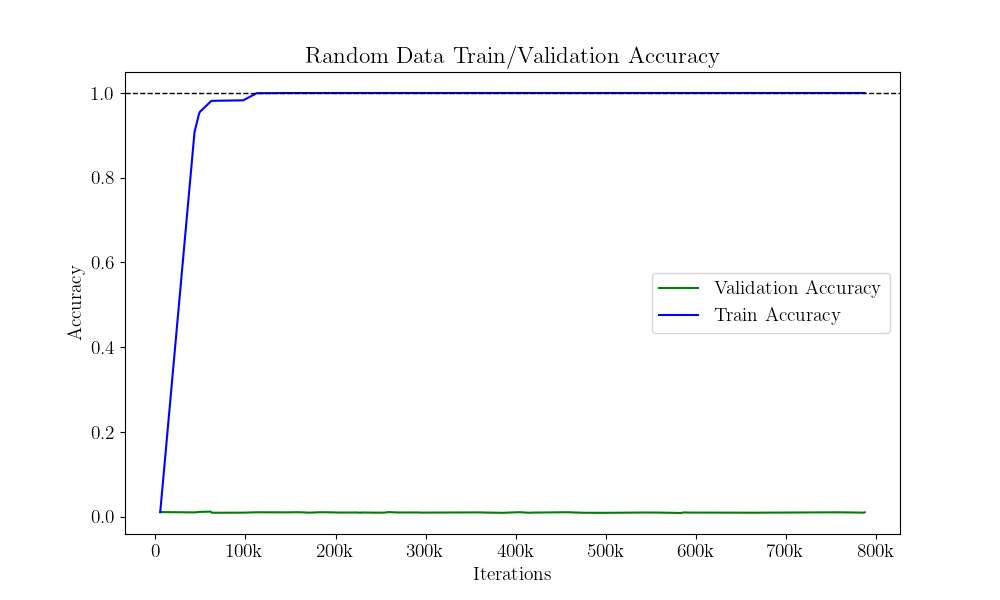
\includegraphics[width=\linewidth,  trim=0 0 0 17mm, clip]{figures/figure_3_1_random_data_run.png}
    \end{subfigure}
    \hfill
    \begin{subfigure}{0.975\linewidth}
        \centering
        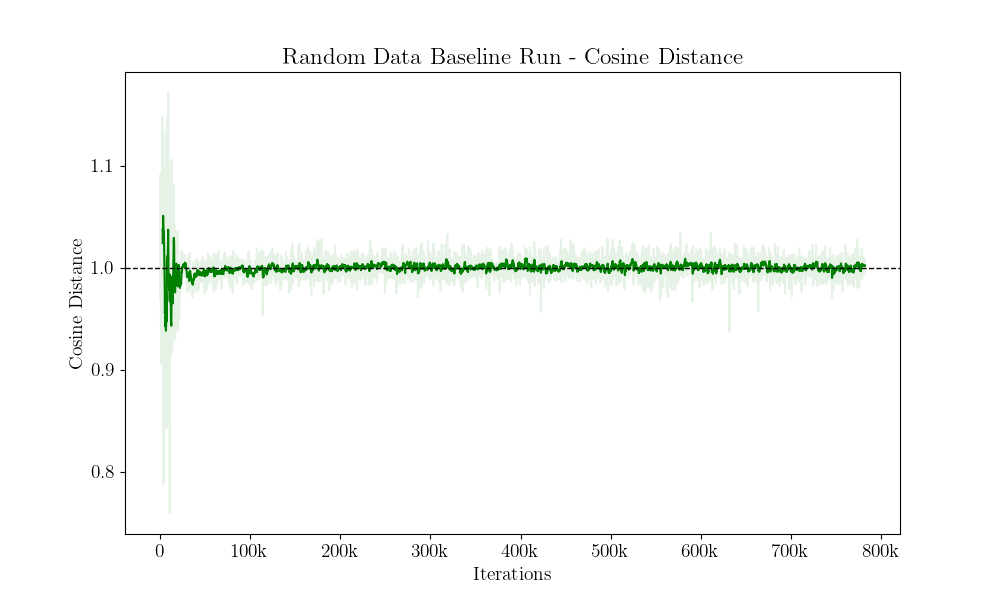
\includegraphics[width=\linewidth,  trim=0 0 0 17mm, clip]{figures/figure_3_2_Random_Data_Run_Cosine_Distance.png}
    \end{subfigure}
   
    \caption{Train and validation accuracy (top) and the cosine distance between micro-gradients (bottom) with rolling average in dark green and raw values in light green, over iterations of a baseline training ResNet18 without GAF on random noise. The model overfits, reaching 100\% training accuracy, but the micro-gradients cosine distance remains above 0.96 throughout the entire training, and above 0.99 for all iterations after the very early iterations. }
    \label{fig:random_data_run}
\end{figure}



With Gradient Agreement Filtering (GAF), instead of blindly averaging all micro-gradients in $\mathcal{M}$, we apply a cosine distance threshold to select only those micro-gradients that are aligned within a given threshold $\tau$, as shown in \Cref{alg:gaf}. Let $\mathbf{g}_i = \nabla_\theta \mathcal{L}(\mathcal{U}_i; \theta)$ denote the micro-gradient for microbatch $\mathcal{U}_i$. The cosine distance between a candidate micro-gradient $\mathbf{g}_i$ and the running sum of accepted gradients $\mathbf{g}$ is $D_c(\mathbf{g}_i, \mathbf{g})$.

We compute a rolling aggregation of micro-gradients starting from the local gradient $\mathbf{g}$ and then checking one by one, and only including those for which $D_c(\mathbf{g}_i, \mathbf{g}) \leq \tau$. We keep a counter $c$ of the agreed upon gradients starting at $c = 1$. Each accepted gradient $\mathbf{g}_i$ is added to the running sum $\mathbf{g}$, and our count $c$ is incremented to keep track of the number of accepted gradients. The filtered macrobatch gradient is
\begin{equation} \label{eq:gaf_grad_update}
   \nabla_\theta \mathcal{L}_{\text{GAF}}(\mathcal{M}; \theta) = \mathbf{g}_{\text{GAF}} = \frac{\mathbf{g}}{c}.
\end{equation}

If no two gradients meet the threshold $\tau$ then $c = 1$ and we skip the update without modifying the optimizer or scheduler as we do not have consensus of any two micro-gradients. Otherwise, the GAF-based SGD update is
\begin{equation}
    \theta \leftarrow \theta - \eta \mathbf{g}_{\text{GAF}}.
\end{equation}

Note, that this implementation is order dependent so could be susceptible to degenerate examples. For example if the initial micro-gradient is orthogonal to all others, then none will agree and the entire macrobatch will be skipped and wasted. This is a shortcoming that could be addressed by tweaking the AllReduce algorithm such that each microgradient acts as the ``initial'' micro-gradient starting from its home GPU, and goes around the ring. The summed micro-gradient with the largest (or smallest) agreement could be the one that is then AllGather'd to the rest of the GPUs. We leave possible implementation to future research. 

% Finally, it is possible to derive that for sufficiently small step size $\eta$, the validation loss and generalization error will be monotonically non-increasing with every GAF step. Such a bound is not possible with standard SGD. If we assume that all samples in the training and validation datasets are sampled i.i.d, and the gradient of our loss function $\nabla_{\theta} \mathcal{L}^{\text{val}}_{\theta}$ is Lipschitz continuous with Lipschitz constants $L \geq 0$, then for a given $\tau$ it is possible to choose an $\eta$ such that our validation loss and generalization error will never increase throughout training. Specifically, if we assume that all samples in the train and validation set are sampled i.i.d, and that the gradient of our loss function  \( \nabla \mathcal{L}^{\text{val}}_{\theta} \) is Lipschitz continuous with Lipschitz constant \( L \geq 0 \), then if we choose a $\tau$ and $\eta$ such that the following inequality always holds: 

% % \[
% % \eta \leq \frac{2 \| g_{\text{batch1}} \| \cos\theta }{L \| g_{\text{batch2}} \| } \leq \frac{2 (1 - \tau) }{L},
% % \]
% \[
% \eta \leq \frac{2 (1 - \tau) }{L},
% \]

% then, every GAF step is guaranteed to maintain or improve validation loss and generalization error. To show how practical this bound is, we empirically estimate L for our architectures to be between 20 and 200. So if we select a $\tau = 0.95$, then if we use a starting $\eta <= 5 \times 10^{-4}$ every step will guarantee a non-increasing validation loss and generalization error. This is exactly what we observe in \Cref{fig:cifarn_does_not_overfit_plot} when we train with $\tau = 0.95$, and set our initial learning rate to $\eta = 5 \times 10^{-4}$. 

% For a complete proof, please see the Appendix. This brings into question whether or not we still need a validation set at all in SGD. 

% With Gradient Agreement Filtering (GAF), instead of blindly averaging all micro-gradients in $\mathcal{M}$, we apply a cosine distance threshold to select only those micro-gradients that are aligned within a given threshold $\tau$ as show in \Cref{alg:gaf}. Let $\mathbf{g}_i = \nabla_\theta \mathcal{L}(\mathcal{U}_i; \theta)$ and $\mathbf{g}_j = \nabla_\theta \mathcal{L}(\mathcal{U}_j; \theta)$ denote the micro-gradients for microbatches $\mathcal{U}_i$ and $\mathcal{U}_j$, respectively. Then, the cosine distance between these micro-gradients is defined by $D_c(\mathbf{g}_i,\mathbf{g}_j)$.

% We compute a rolling aggregation of microgradients sampling one $D_c(\mathbf{g}_i,\mathbf{g}_j) \leq \tau$ with at least one other $\mathcal{U}_i$. The filtered macrobatch gradient is then calculated as
% \begin{equation} \label{eq:gaf_grad_update}
%     \mathbf{g}_{\text{GAF}} = \nabla_\theta \mathcal{L}_{\text{GAF}}(\mathcal{M}; \theta) = \frac{1}{c} \sum_{\mathbf{g} \in \mathcal{G}} \mathbf{g}.
% \end{equation}
% If $|\mathcal{G}|=0$ we just skip the update and do not update our optimizer or scheduler. 

% The GAF-based SGD update is then
% \begin{equation}
%     \theta \leftarrow \theta - \eta \nabla_\theta \mathcal{L}_{\text{GAF}}(\mathcal{M}; \theta).
% \end{equation}
